\chapter{Methodology}\label{ch:methodology}

\section{Software Development Life Cycle}
The process of making software applications is like building something step by step. One common way to do this is called the Software Development Life Cycle (SDLC). It's a structured method to create software that's efficient, effective, and meets what users need.This model is great for managing risks, being flexible, and always making things better as you go along. Using the Spiral Model for making the Medical Report Scanning App has many benefits. It helps make sure everything is well-organized, lets us manage any problems that might come up, and allows us to keep improving the app as we work on it.

\begin{figure}[h]
    \centering
    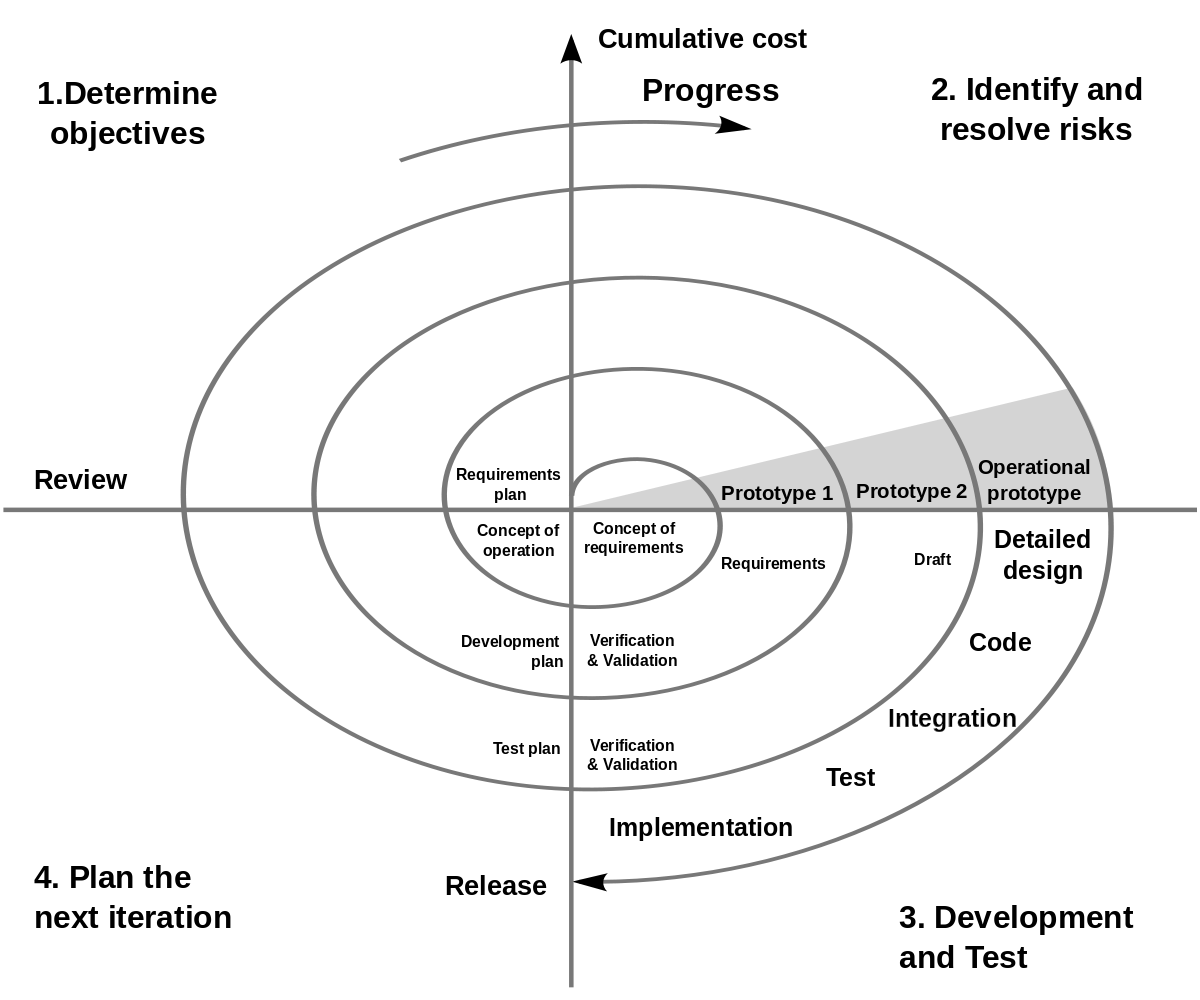
\includegraphics[width =150mm]{figures/spiral_model.png}
    \caption{Spiral Model}
\end{figure}

\subsection*{Identification and Requirement Gathering}
During this phase, the project's objectives, requirements are defined. The goals of the Medical Report Scanning  App, such as OCR integration, AI categorization, and secure data management, are outlined. User needs are identified, and a preliminary scope is defined.
\subsection*{Risk Analysis}
In this phase, potential risks and challenges associated with the app's development are assessed. Risks related to integrating OCR and AI technologies, data security, and user adoption are identified. Strategies for mitigating these risks are developed, allowing for informed decision-making.
\subsection*{Development}
The development phase focuses on creating the app's core functionalities. Using the Spiral Model's iterative approach, the app's features, such as document scanning, AI categorization, and report retrieval, are developed in incremental cycles. Each cycle results in a more refined and functional version of the app.
\subsection*{Evaluation}
At the end of each development cycle, a thorough evaluation of the app's progress is conducted. Stakeholders, including healthcare professionals and users, provide feedback on the app's usability, functionality, and performance. This feedback guides improvements and refinements in subsequent cycles.
\subsection*{Planning}
Based on the evaluation results, plans for the next cycle are refined and adjusted. Changes in requirements, user feedback, and emerging risks are incorporated into the development roadmap. This adaptive planning ensures that the app remains aligned with user needs and project goals.
\subsection*{Deployment}
Once the app reaches a mature stage with all intended features, it undergoes thorough testing and quality assurance. The final product is deployed to a limited user group for a pilot test, allowing for real-world validation and identifying any remaining issues.
\subsection*{Maintenance and Enhancement}
After deployment, the app enters the maintenance phase, where ongoing support, bug fixes, and updates are provided. User feedback and evolving needs are addressed through continuous enhancements, ensuring the app remains relevant and effective.

\section{System Development Tools}
\subsection*{}
\subsection*{Mongodb}
MongoDB serves as an agile and scalable NoSQL database solution for the Medical Report Scanning  App, thanks to its document-oriented structure that accommodates diverse medical report formats. With dynamic schema support, MongoDB flexibly manages changing data needs, while its efficient indexing and querying enable quick access to specific reports. MongoDB's seamless integration with Node.js and React Native facilitates development, and its security features, including encryption and access control, safeguard sensitive patient data. Overall, MongoDB's versatility and compatibility contribute to efficient medical report management and enhanced user experiences within the app.
\subsection*{Node.js}
Node.js, powered by Chrome's V8 engine, is a versatile runtime environment crucial to the Medical Report Scanning and Organization App's development. By using JavaScript for both frontend and backend development, Node.js offers unified coding. Its extensive package ecosystem and npm support streamline development and code reuse, while integration with React Native ensures smooth component communication. Ultimately, Node.js contributes to the app's high performance, scalability.
\subsection*{Express.js}
Express.js, which works together with Node.js, is like a powerful tool for the backend of the Medical Report Scanning App. It helps make things work smoothly and efficiently. It simplifies creating connections between the app's front part and the database behind the scenes.  It has a lot of helpful tools that speed up the app's development, making it easier to add useful features like user logins, checking data, and handling errors. Express.js makes the app's backend work really well, making it fast, able to handle many users, and responsive.
\subsection*{React Native}
React Native is a powerful tool for building mobile apps, like the Medical Report Scanning and Organization App. It's  a versatile framework that allows developers to create apps that work on both Android and iOS devices using just one codebase. This means less work and more efficiency. React Native takes care of making the app look and feel right on different devices, so users get a consistent experience. It also lets developers use JavaScript, a popular programming language, for building both the app's front part that users see and the back part that handles data. This makes development faster and more organized. With React Native, the Medical Report Scanning  App can be built quickly, look great, and work well on different devices, making it a smart choice for creating a user-friendly and effective app.
\subsection*{Git and Github}
Git is a version control system that lets you manage and keep track of your source code history. GitHub is a cloud-based hosting service that lets you manage Git repositories.For the development of the Medical Report Scanning App, Git and GitHub provide invaluable advantages. Different team members can work on distinct parts of the app simultaneously, making progress without stepping on each other's toes. Any changes made can be tracked, allowing for easy identification of who did what and when.
\subsection*{Optical Character Recognition (OCR)}
Optical Character Recognition (OCR) is a  technology  that can recognize and understand text from images or scanned documents. OCR is a powerful tool that transforms pictures of words into editable and searchable text, making it easy to manage and use information. For the app, OCR acts as a smart translator, converting physical medical reports into digital text that can be searched, sorted, and shared. This users can quickly find specific information they need without flipping through piles of paper.








